
\chapter{四足機器人}
%--------------------應用範圍反作用--------------------%
\section{應用範圍及作用}
四足機器人為一種模仿動物四肢運動方式的機器人,分別由四組步行機構及本體組成,利用電子元件驅動機械臂進行運動,可用以替代人力執行任務,同時為人們帶來許多樂趣及益處。可大致上分為以下幾項:\
\begin{enumerate}
\item 軍事:四足機器人有良好的機械性能,搭配著電子控制系統,可以輕鬆在各地形中運輸物品及人員,透過感測器的回饋,調適馬達的行程及出力大小,在戰場中穿梭及運輸補給品,或是在搜救行動也可以當作先鋒隊,減少搜救人員的危險性並增加搜救的效率。\
\item 工業:減少作業人員在高風險環境中造成職業傷害,並保持高效的運作,減少工業中的資源浪費。\
\item 民生:可以執行各種控制指令,可以體驗仿生機器人的操作特性和樂趣,也可以幫助幫運重物,許多人們也會依照需求進行各式改裝及編程,讓四足機器人可以達到所需的功能。\
\end{enumerate}
隨著電腦的普及,各式各樣的編程軟體如雨後春筍般誕生,並且計算機語言也日益精簡,讓更多使用者可以輕而易舉的使用,網路上也有許多工程師分享開源的程式可以參考及學習,配合現在AI的發展,四足機器人應用範圍越加的廣泛,正因為如此我們才以四足機器人為主題,研究其誕生到成品將會有哪些的分析及考量。\\[6pt]
\newpage
%----------------步行結構運動學模型介紹---------------%
\section{步行結構運動學模型介紹}

在步行結構設計之初,通常透過模仿生物,來創造不同的機械模型,不同型態的機械模型都有其各自特性,對於連接機構的運動控制,一般來說,腿部的機械結構不能過於複雜,過多的機械零件需要較精細的控制元件及設計,對於控制運動軌跡及製作成本來說較不益,以下為Goegebra所繪製連桿機構講述:\
\begin{enumerate}
\item 三連桿閉環機構:
此三連桿閉環機構(圖3.1.1)為三個聯桿及三顆馬達組成,此以一個關節連接本體,此種機構優點在於結構較為緊湊、簡單,通過三連桿關節的旋轉角度控制尾端的位置,達到目標動作及整體姿態,具有靈活性、反應快速、定位精度高等優點。\

\begin{figure}[hbt!]
\begin{center}
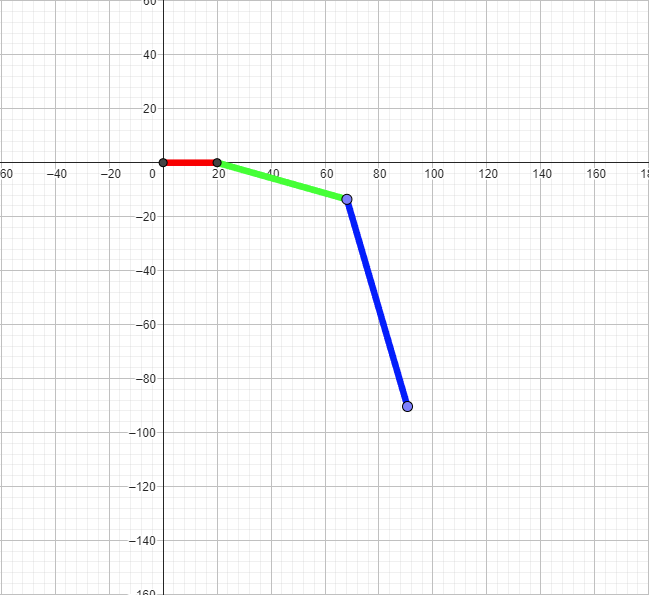
\includegraphics[width=14cm]{三連桿閉環機構}
\caption{\Large 三連桿閉環機構}\label{三連桿閉環機構}
\end{center}
\end{figure}
\newpage

\item 四連桿閉環機構:
此四連桿閉環機構(圖3.1.2)為兩個聯桿及兩顆馬達組成,為四個結構連桿組成一個不規則四邊形,有著兩個馬達分別驅動Leg1-5(綠)及Leg2(紅)桿件搖擺,可以讓連桿有大幅度的運動,此機構較為複雜,需要精細的控制才能實現較穩定的運動,但有著能承受較大負載的優勢,對於運動穩定性也有著良好的表現,也是這個專題研究為何會選擇此機構的原因之一。
\end{enumerate}

\begin{figure}[hbt!]
\begin{center}
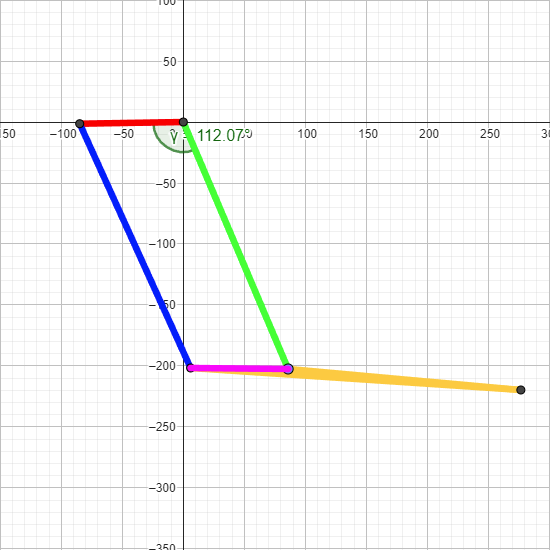
\includegraphics[width=14cm]{步行機構ggb}
\caption{\Large 四連桿閉環機構}\label{GeoGebra步行機構}
\end{center}
\end{figure}
\newpage

%----------------硬體架構---------------%
\section{硬體架構}

\begin{figure}[hbt!]
\begin{center}
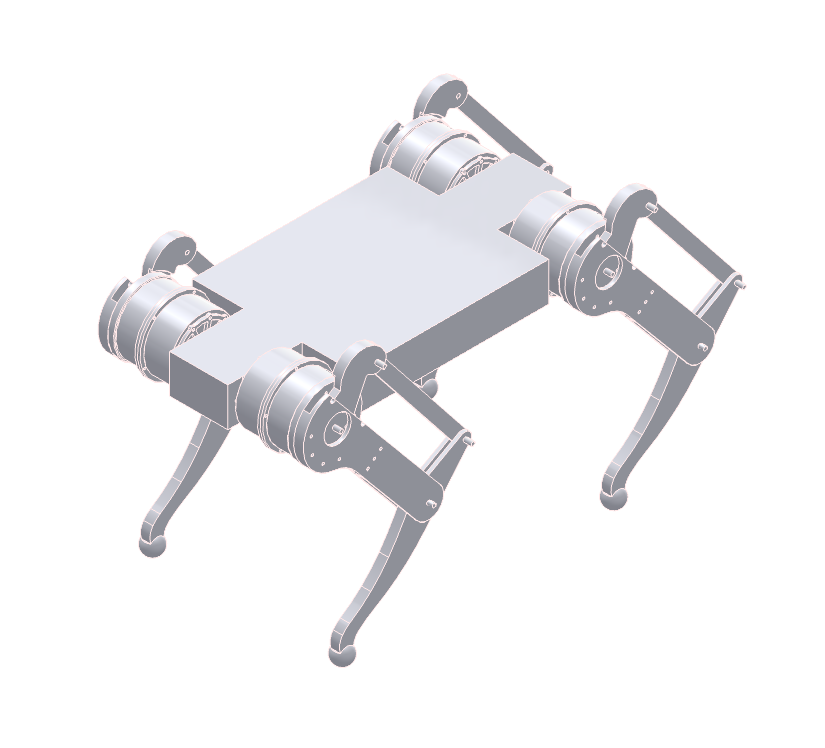
\includegraphics[width=\textwidth]{四足機器狗}
\caption{\Large 四足機器人}\label{四足機器狗}
\end{center}
\end{figure}
上圖所示為本次專題研究的有限元素法的分析對象"四足機器人",由四個步行機構及一個本體組成,因其有負重及穩定性的需求,所以使用上述所講的四連桿閉環機構。\
\newpage

\begin{figure}[htbp]
  \begin{minipage}[t]{0.3\linewidth}
    \centering
    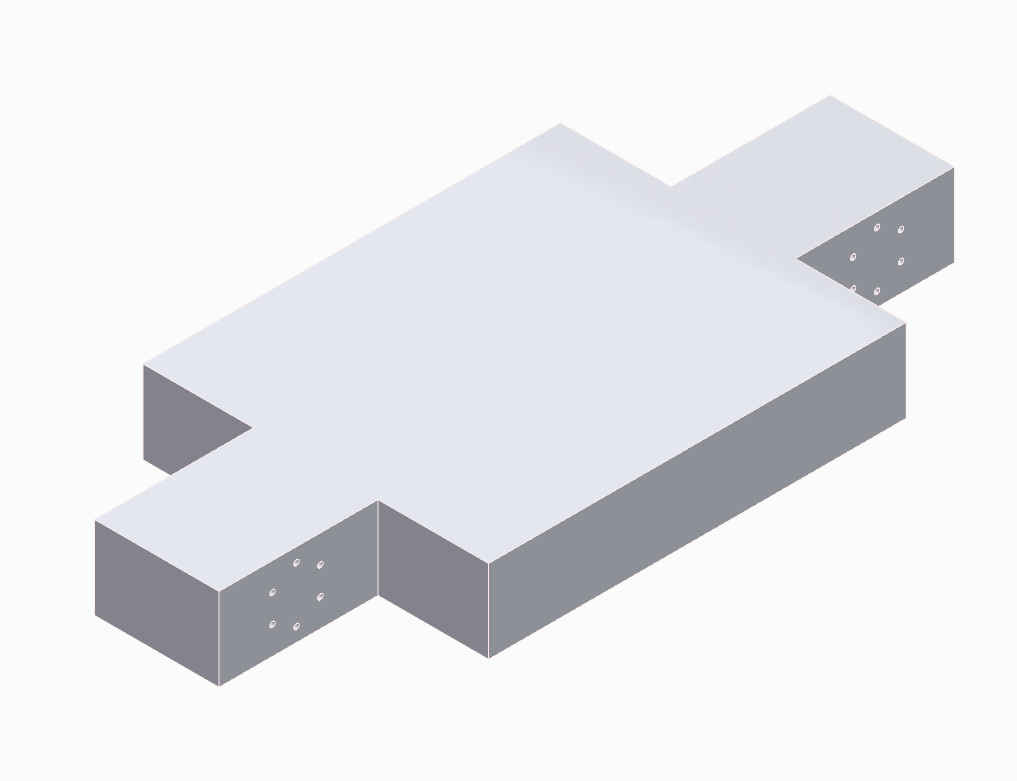
\includegraphics[height=3.5cm,width=3.5cm]{本體}
    \caption{本體}
    \label{本體}
  \end{minipage}
  \hfill
  \begin{minipage}[t]{0.3\linewidth}
    \centering
    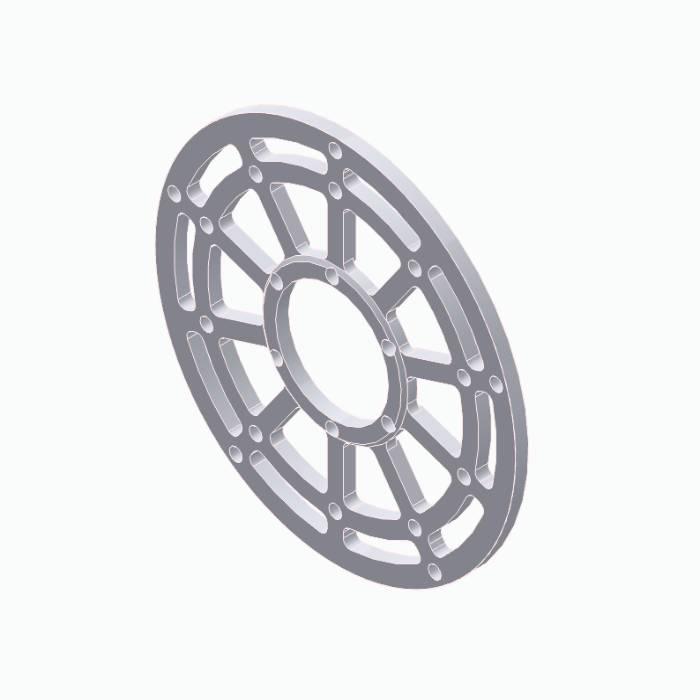
\includegraphics[height=3.5cm,width=3.5cm]{馬達連接座}
    \caption{連接座}
    \label{馬達連接座}
  \end{minipage}
  \hfill
  \begin{minipage}[t]{0.3\linewidth}
    \centering
    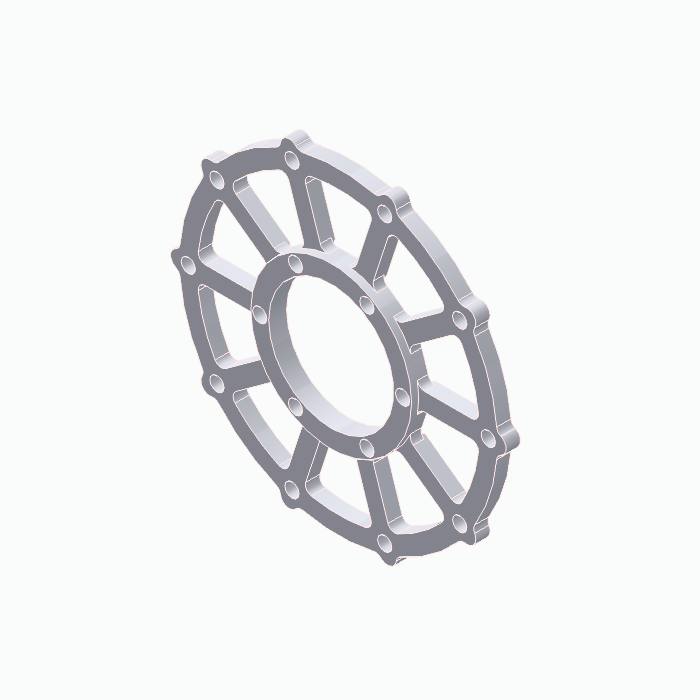
\includegraphics[height=3.5cm,width=3.5cm]{馬達連接座-2}
    \caption{連接座-2}
    \label{馬達連接座-2}
  \end{minipage}
\end{figure}

\begin{figure}[htbp]
  \begin{minipage}[t]{0.3\linewidth}
    \centering
    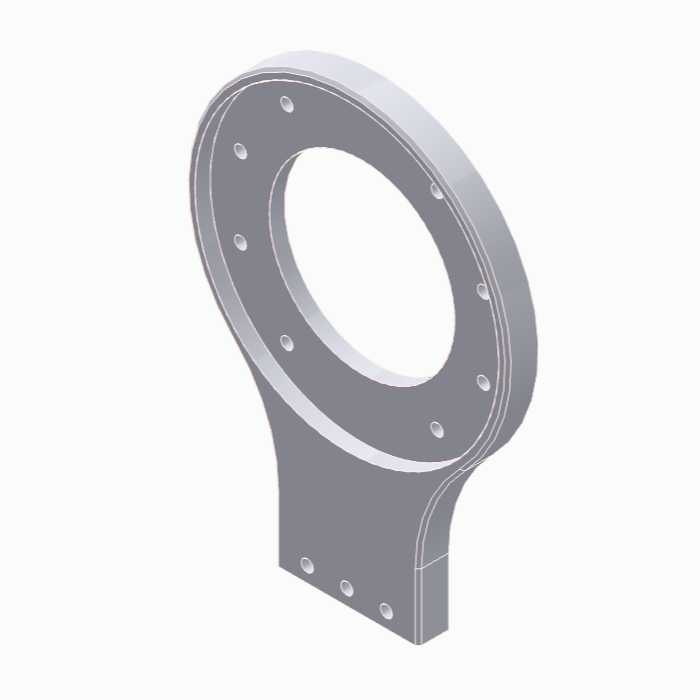
\includegraphics[height=3.5cm,width=3.5cm]{leg1-1}
    \caption{Leg1-1}
    \label{leg1-1}
  \end{minipage}
  \hfill
  \begin{minipage}[t]{0.3\linewidth}
    \centering
    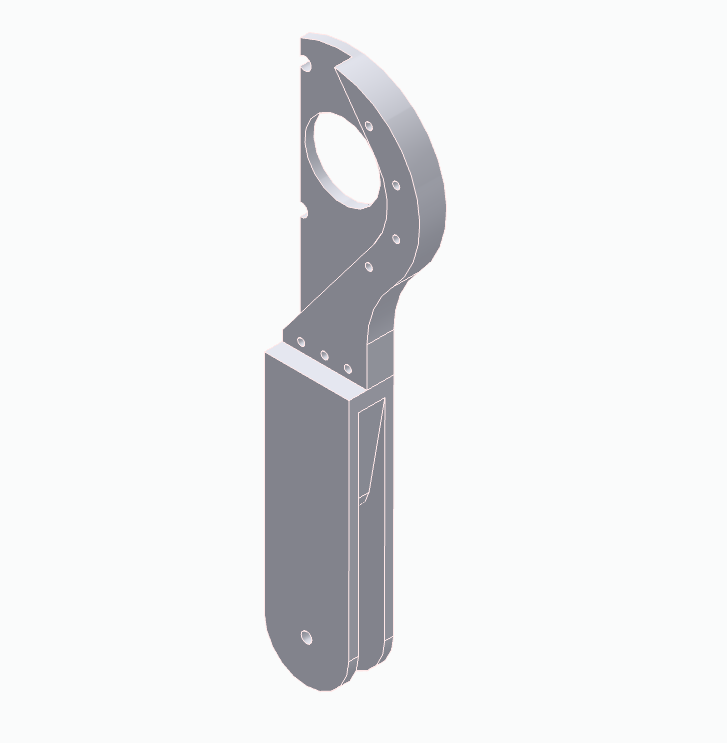
\includegraphics[height=3.5cm,width=3.5cm]{leg1-5}
    \caption{Leg1-5}
    \label{leg1-5}
  \end{minipage}
  \hfill
  \begin{minipage}[t]{0.3\linewidth}
    \centering
    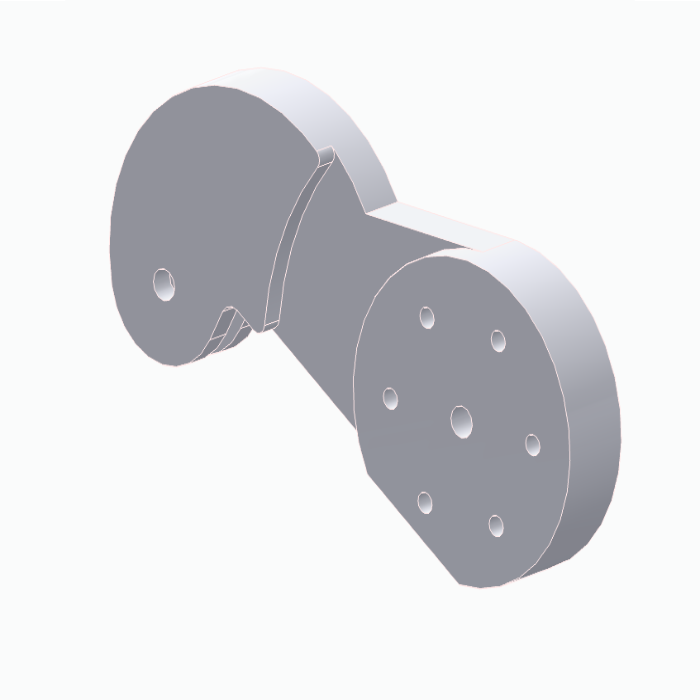
\includegraphics[height=3.5cm,width=3.5cm]{leg2}
    \caption{Leg2}
    \label{leg2}
  \end{minipage}
\end{figure}

\begin{figure}[htbp]
  \begin{minipage}[t]{0.3\linewidth}
    \centering
    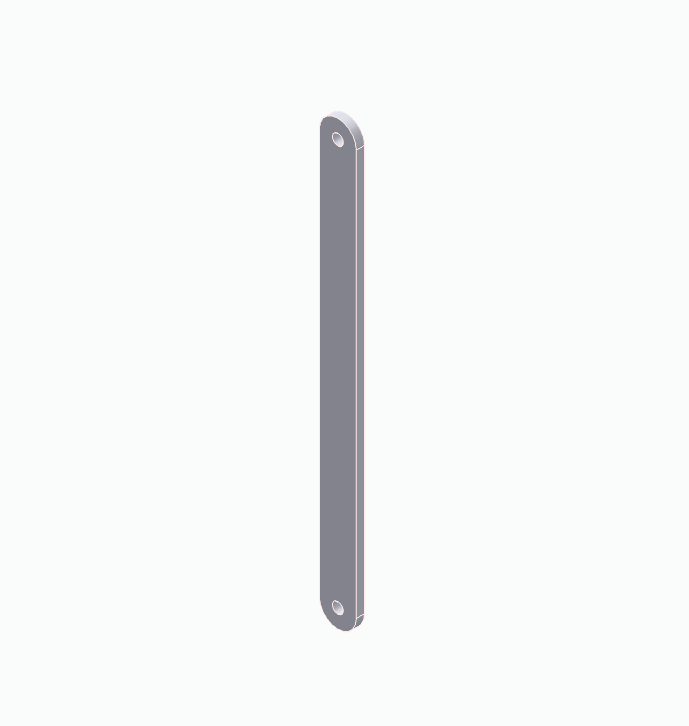
\includegraphics[height=3.5cm,width=3.5cm]{leg3}
    \caption{Leg3}
    \label{leg3}
  \end{minipage}
  \hfill
  \begin{minipage}[t]{0.3\linewidth}
    \centering
    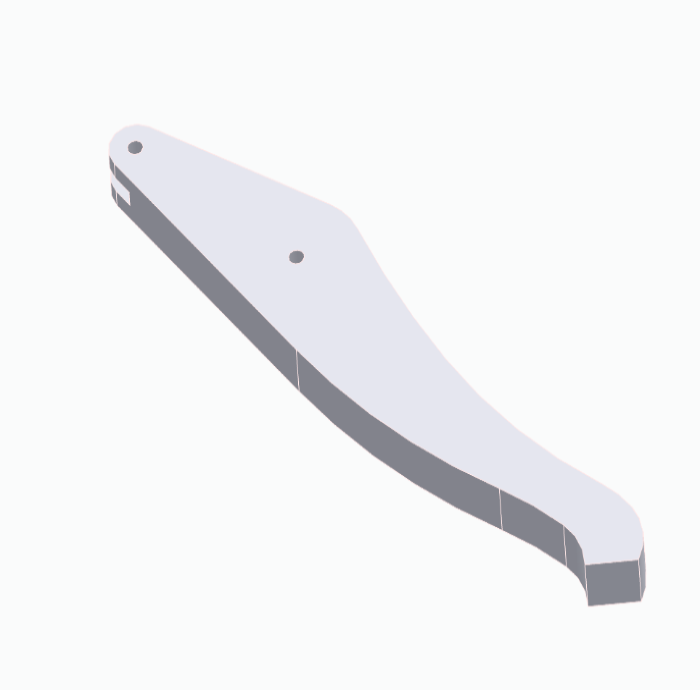
\includegraphics[height=3.5cm,width=3.5cm]{leg4}
    \caption{Leg4}
    \label{leg4}
  \end{minipage}
  \hfill
  \begin{minipage}[t]{0.3\linewidth}
    \centering
    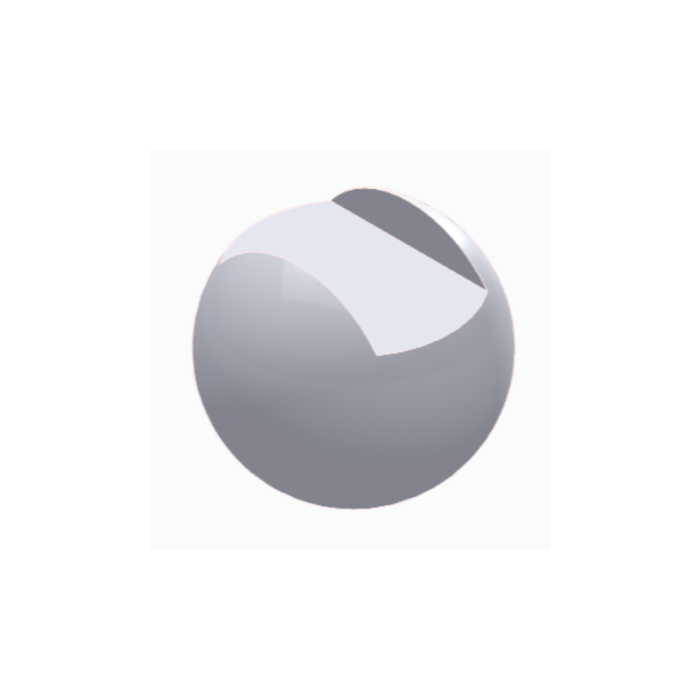
\includegraphics[height=3.5cm,width=3.5cm]{leg6}
    \caption{Leg6}
    \label{leg6}
  \end{minipage}
\end{figure}

\begin{figure}[htbp]
  \centering
  \begin{minipage}{0.3\textwidth}
    \centering
    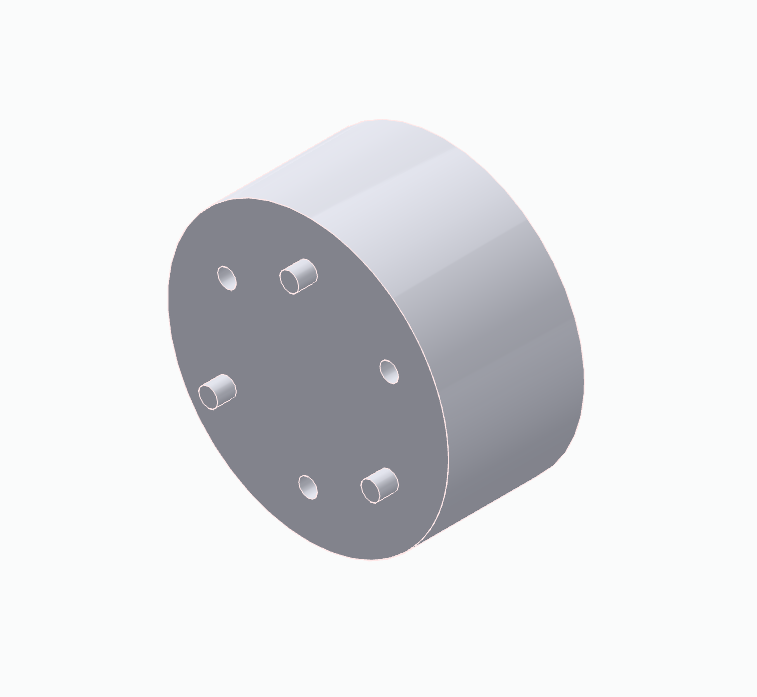
\includegraphics[width=\textwidth]{馬達軸}
    \caption{馬達軸}
    \label{馬達軸}
  \end{minipage}
  \hfill
  \begin{minipage}{0.3\textwidth}
    \centering
    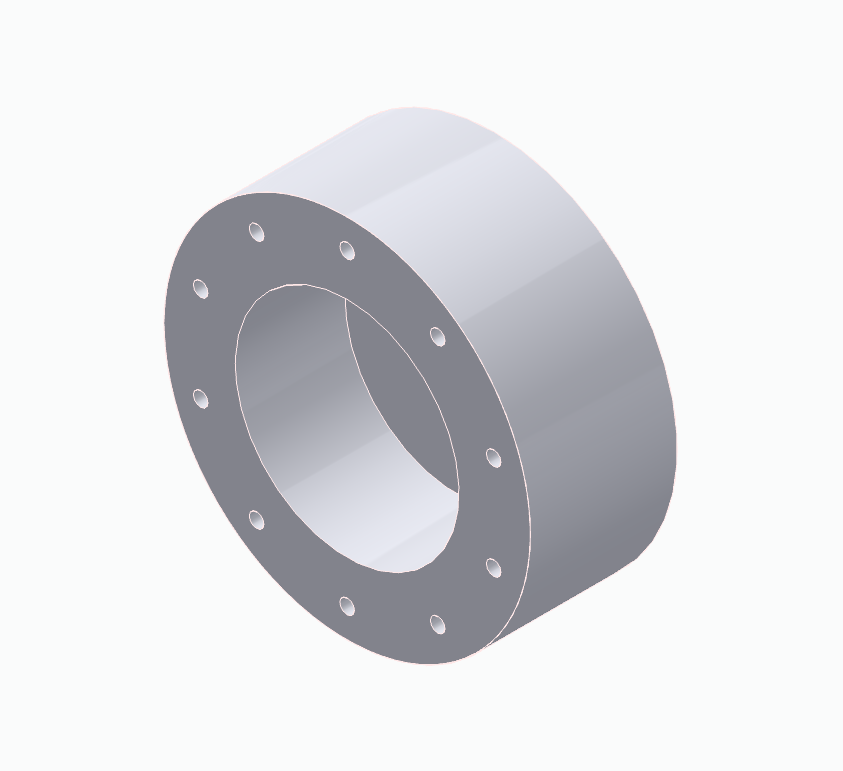
\includegraphics[width=\textwidth]{馬達底座}
    \caption{馬達底座}
    \label{馬達底座}
  \end{minipage}
 \end{figure}
\newpage

%-------------四連桿機構運動學模型---------------%
\section{四連桿機構運動學模型}

四連桿機構最早可以追朔到19世紀末的機械工程領域,用於織布機的機械結構,由四個桿件及四個轉動連接點組成,形成一個不規則的四邊形閉環,可以控制機械的運動軌跡及速度,實現自動化編織過程。\
在現代,四連桿閉環機構被廣泛用於機械工業、機器人技術等領域。作為機器人的關節結構有靈活、平穩、高負載、高自由度等特性,使成為此領域重要結構之一,隨著科技的發展人們也不斷對此機構進行改進和創新、優化以滿足更多的應用需求。\
此順向運動學將對步行機構(圖.3.15)(圖.3.16)進行計算,由於四組步行機構為相同模型,因此只要提出一個計算即可。\\
\begin{figure}[htbp]
  \begin{minipage}[t]{0.45\linewidth}
    \centering
    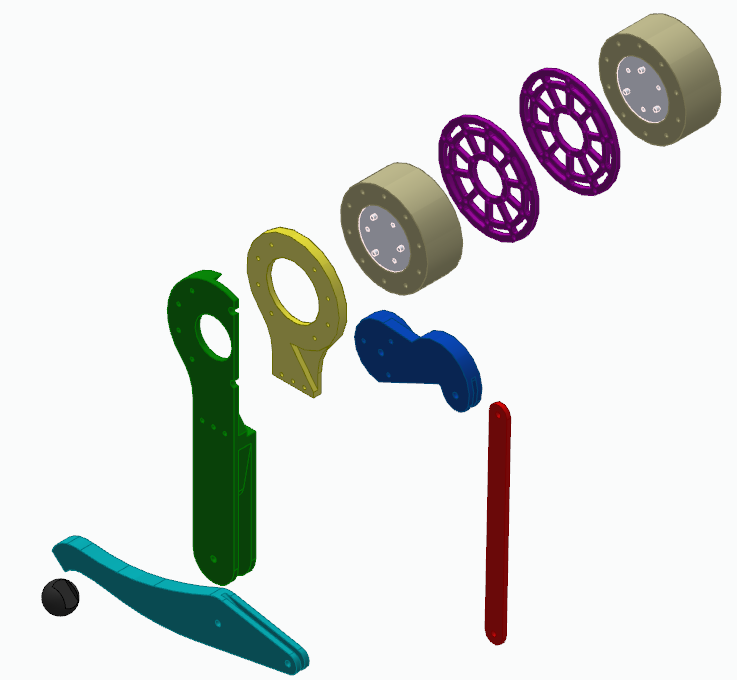
\includegraphics[height=5cm,width=5cm]{步行機構分解圖}
    \caption{步行機構分解圖}
    \label{步行機構分解圖}
  \end{minipage}
  \hfill
  \begin{minipage}[t]{0.45\linewidth}
    \centering
    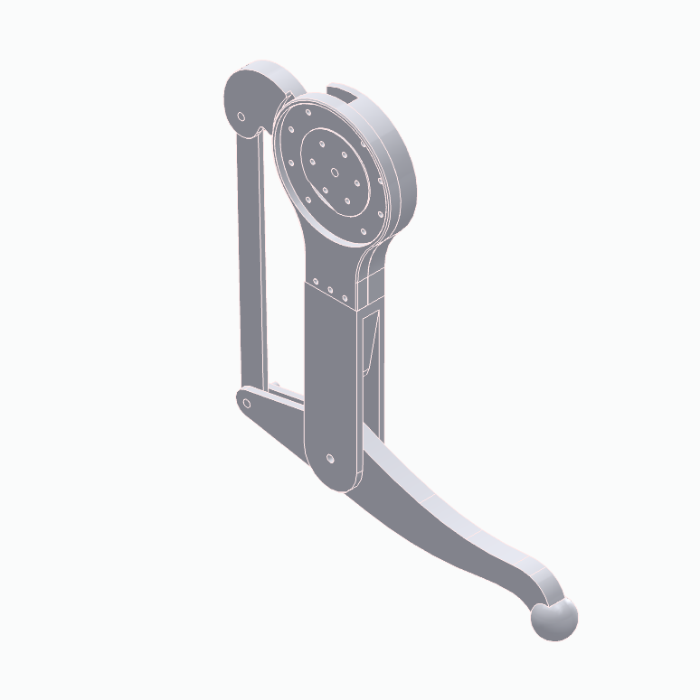
\includegraphics[height=5cm,width=5cm]{步行機構}
    \caption{步行機構}
    \label{步行機構}
  \end{minipage}
\end{figure}
\newpage

\begin{figure}[htbp]
  \begin{minipage}[t]{0.5\linewidth}
    \centering
    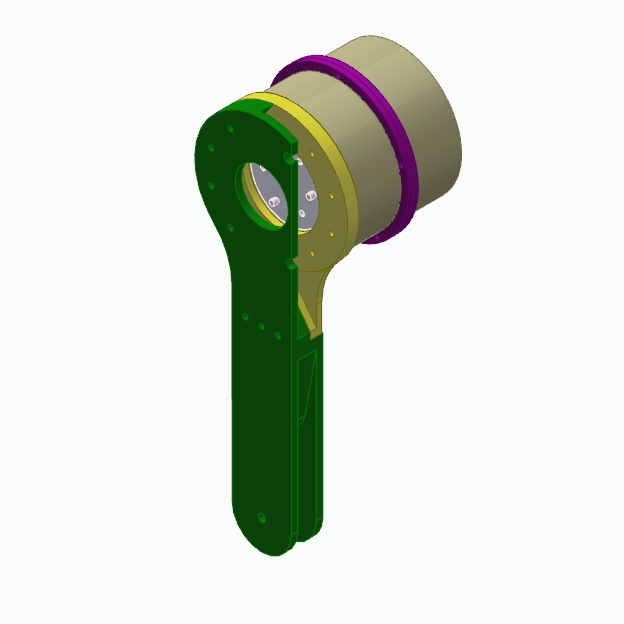
\includegraphics[height=6cm,width=6cm]{馬達(一)控制件}
    \caption{馬達(一)}
    \label{馬達(一)控制件}
  \end{minipage}
  \hfill
  \begin{minipage}[t]{0.5\linewidth}
    \centering
    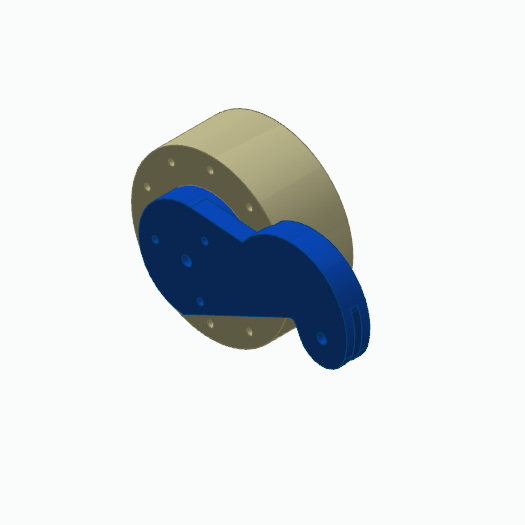
\includegraphics[height=6cm,width=6cm]{馬達(二)控制件}
    \caption{馬達(二)}
    \label{馬達(二)控制件}
  \end{minipage}
\end{figure}

將連桿分為兩部分\\
A部分:由馬達(一)所控制的結構為零件Leg1-1(黃)和Leg1-5(綠)。\
B部分:由馬達(二)所驅動的結構為零件Leg2(藍)。\
連桿Leg3(紅)B部份所控制,被動對Leg4(青)施以推力及拉力,因此Leg4(青)中間受A部分連桿約束後將會控制Leg6(橡膠套)做動。\\


\begin{figure}[hbt!]
\begin{center}
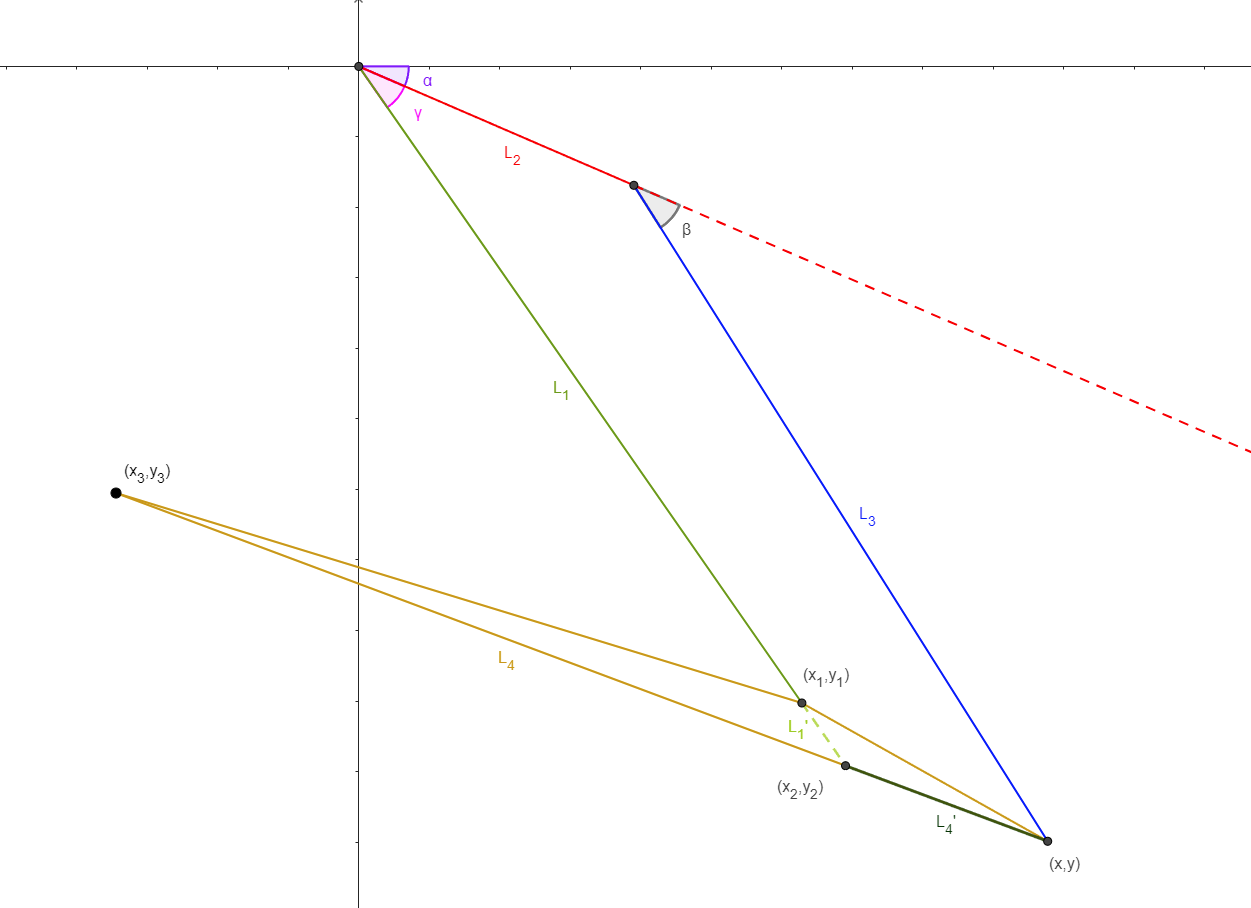
\includegraphics[angle=90,width=10cm]{Forward kinematics formula}
\caption{\Large 連桿圖}\label{Forward kinematics formula}
\end{center}
\end{figure}

可見A部分為二連桿機構組成,因此使用三角函數即可分別計算出末端點的相對座標位置,因此可以繪出連桿圖及列出算式如下:\
(X,Y)座標
\[
\begin{aligned}
x&=L_{2}\cos \alpha +L_{3}\cos \left( \alpha +\beta \right)\\
y&=L_{2}\sin \alpha +L_{3}\sin \left( \alpha +\beta \right)\\
\end{aligned}
\]

B連桿部份則為單支連桿組成,套入三角函數的計算方式如下:\\
\[
\begin{aligned}
x_{1}&=L_{1}\cos \left( \alpha +\theta \right)\\
y_{1}&=L_{1}\sin \left( \alpha +\theta \right)\\
\end{aligned}
\]

求出A部分(x,y)座標連接到末端點($\x_{3}$,$\y_{3}$),再以內分點公式求出$\L_{1}$延伸至$\L_{4}$之焦點:\\
$\L_{4}$:為($\x_{3}$,$\y_{3}$)$至($\x_{1}$,$\y_{1}$)長度
$\L_{4}'$:為($\x_{2}$,$\y_{2}$)至(x,y)長度

\[
\begin{align*}
x_{2}&= \frac{(L_{1} + L_{1}') \x_{1}}{L_{1}} \\
y_{2}&= \frac{(L_{1} + L_{1}') \y_{1}}{L_{1}}
\end{align*}
\]
找出點(x,y)及點($\x_{2}$,$\y_{2}$)即可使用內分點公式求出末段點與地面之交點:\\
\[
\begin{align*}
x_{3}&= \frac{(L_{4} \x_{2} - (L_{4} - L_{4}') \x}{L_{4}'} \\
y_{3}&= \frac{(L_{4} \y_{2} - (L_{4} - L_{4}') \y}{L_{4}'}
\end{align*}
\]
由此公式得出目標末端點相對至基座連結關節座標,以利於控制\\

\subsection{逆向運動學}
跟順向運動學不同是,此種求解方法需要先定義目標位置和姿態,通過觀察機械系統的末端推導出機械系統中各關節的運動及整理姿態,通常可以以一個非線性方程組問題表示,其中每個方程都可代表著一個機械臂關節的末端位置及角度,這些方程一般都是非線性的,因此需要使用數值方法去求解。\
作用於機器人在空間中精準控制末端姿態,在機器臂控制、機器人視覺和機器人運動學等領域有著許多應用的地方。\\

\section{運動軌跡}
以Leg1-5的長度為半徑建立圓形,且給定數值滑桿(一)控制Leg1-5末端點並限制其角度。\
以Leg2的長度為半徑生成Leg2末端點,且給定數值滑桿(2)控制Leg2末端點並限制其角度。\
將兩點設定為搖擺運動,以Leg2末端點為圓心繪製半徑長為Leg3的圓形,再於Leg1-5末端點以L3’為半徑畫圓,即可找出兩圓交點並連接,再用Leg1-5末端點及Leg3末端點為圓心,兩點和目標點距離為半徑畫圓,兩圓交點部分即為目標點。\
由此可得模擬路徑範圍如下圖所示:\\
\begin{figure}[hbt!]
\begin{center}
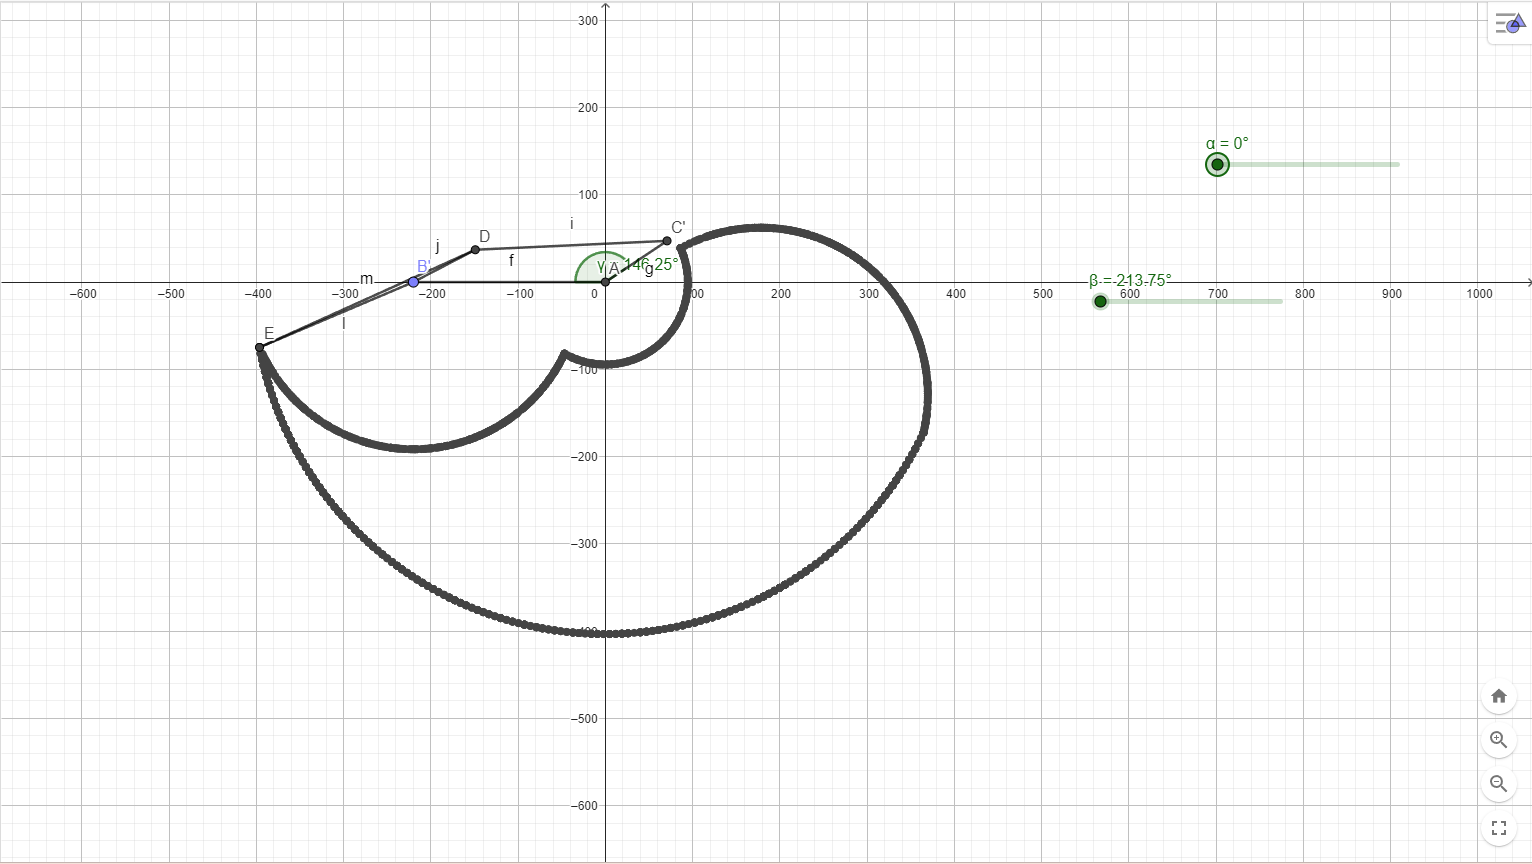
\includegraphics[width=10cm]{機械腿運動軌跡}
\caption{\Large Geogebra運動軌跡}\label{機械腿運動軌跡}
\end{center}
\end{figure}
\newpage
